\documentclass[aspectratio=169]{beamer}

% ==== Theme & basic look ====
\usetheme{Madrid}
\usecolortheme{seahorse}
\setbeamertemplate{navigation symbols}{}
\setbeamertemplate{footline}[frame number]

% ==== Packages ====
\usepackage{amsmath}
\usepackage{amsfonts}
\usepackage{amssymb}
\usepackage{mathtools}
\usepackage{booktabs}
\usepackage{array}
\usepackage{tikz}
\usetikzlibrary{arrows.meta,positioning,calc}
\usepackage{CJKutf8}

% ==== Math shorthand ====
\providecommand{\Tilde}[1]{\tilde{#1}}
\newcommand{\EE}{\mathbb{E}}
\newcommand{\PP}{\mathbb{P}}
\newcommand{\one}{\mathbf{1}}
\newcommand{\Sspace}{\mathcal{S}}
\newcommand{\Aspace}{\mathcal{A}}
\newcommand{\Rspace}{\mathcal{R}}
\newcommand{\red}[1]{\textcolor{red}{#1}}
\DeclareMathOperator*{\argmax}{arg\,max}

% ==== Title page details ====
\title[Reinforcement Learning]{Reinforcement Learning: From Interaction to Temporal-Difference Learning}
\author{Pipi Hu}
\institute[BIMSA]{Beijing Institute of Mathematical Sciences and Applications}
\date{\today}

\pgfdeclareimage[width=2cm]{logo}{../figures/logo.png}
\logo{\pgfuseimage{logo}}

\AtBeginSection[]
{
    \begin{frame}<beamer>{Outline}
        \tableofcontents[currentsection]
    \end{frame}
}

\AtBeginSubsection[]
{
    \begin{frame}<beamer>{Outline}
        \tableofcontents[currentsection,currentsubsection]
    \end{frame}
}

\begin{document}

\begin{frame}
  \titlepage
\end{frame}

\begin{frame}{Primary Reference and Scope}
\small
\textbf{Primary source.} Sutton and Barto, \emph{Reinforcement Learning: An Introduction}, 2nd edition draft.

\vspace{0.6em}
\begin{itemize}
    \item Chapter 1: the reinforcement learning problem and the role of value.
    \item Chapter 3: finite Markov decision processes, returns, policies, and Bellman equations.
    \item Chapter 6: temporal-difference learning, Sarsa, and Q-learning.
    \item Chapter 7: $n$-step methods, TD($\lambda$), and eligibility traces.
    \item Supporting bridge: dynamic programming, Monte Carlo, and generalized policy iteration.
\end{itemize}
\end{frame}

\begin{frame}{A One-Sentence Main Line}
\centering
\Large
Reinforcement learning is the study of \red{how an agent improves a policy from interaction} by estimating \red{long-term value} and using those estimates to change future behavior.
\end{frame}

\begin{frame}{Lecture Roadmap}
\small
\begin{enumerate}
    \item Start with the agent--environment loop.
    \item Formalize the loop as a finite MDP.
    \item Define the objective through return and value functions.
    \item Use Bellman equations to connect current value with future value.
    \item View algorithms as different ways to do backups.
    \item Move from Monte Carlo and dynamic programming to TD learning.
    \item Extend one-step TD to multi-step credit assignment through eligibility traces.
\end{enumerate}
\end{frame}

\section{The Reinforcement Learning Problem}

\begin{frame}{What Makes RL Different?}
\small
\begin{tabular}{>{\raggedright\arraybackslash}p{0.25\textwidth}
                >{\raggedright\arraybackslash}p{0.31\textwidth}
                >{\raggedright\arraybackslash}p{0.31\textwidth}}
\toprule
Setting & Supervised Learning & Reinforcement Learning \\
\midrule
Data & Labeled examples $(x,y)$ & Experience stream $(S_t,A_t,R_{t+1},S_{t+1})$ \\
Feedback & Correct target is visible & Reward is scalar, delayed, and partial \\
Decision effect & Prediction does not change data source & Actions change future states and data \\
Goal & Minimize prediction loss & Maximize long-term return \\
\bottomrule
\end{tabular}

\vspace{0.9em}
\textbf{Core difficulty:} the agent must learn from consequences of its own behavior.
\end{frame}

\begin{frame}{Agent--Environment Interface}
\centering
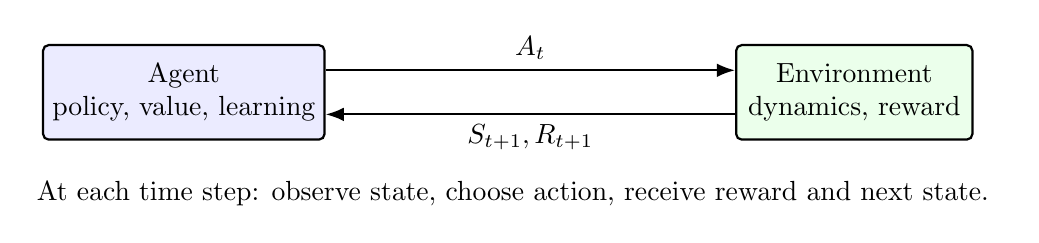
\begin{tikzpicture}[
    box/.style={draw, rounded corners=2pt, minimum width=3.0cm, minimum height=1.2cm, align=center, thick},
    arrow/.style={-Latex, thick}
]
\node[box, fill=blue!8] (agent) {Agent\\policy, value, learning};
\node[box, fill=green!8, right=5.2cm of agent] (env) {Environment\\dynamics, reward};
\draw[arrow] ([yshift=0.28cm]agent.east) -- node[above] {$A_t$} ([yshift=0.28cm]env.west);
\draw[arrow] ([yshift=-0.28cm]env.west) -- node[below] {$S_{t+1}, R_{t+1}$} ([yshift=-0.28cm]agent.east);
\node[below=1.0cm of $(agent)!0.5!(env)$, align=center] {
At each time step: observe state, choose action, receive reward and next state.
};
\end{tikzpicture}
\end{frame}

\begin{frame}{Four Elements of an RL Agent}
\small
\begin{itemize}
    \item \red{Policy} $\pi$: the agent's behavior rule, often $\pi(a\mid s)$.
    \item \red{Reward signal} $R_{t+1}$: immediate feedback that defines the task.
    \item \red{Value function} $v_\pi, q_\pi$: prediction of long-term reward.
    \item \red{Model} $p(s',r\mid s,a)$: optional prediction of environment response.
\end{itemize}

\vspace{0.8em}
\begin{block}{The key distinction}
Reward says what is good immediately. Value estimates what is good after future consequences are considered.
\end{block}
\end{frame}

\begin{frame}{Reward Is Not the Same as Value}
\small
\begin{columns}[T,onlytextwidth]
\begin{column}{0.48\textwidth}
\textbf{Immediate reward}
\begin{itemize}
    \item A scalar signal after one transition.
    \item Defines the objective externally.
    \item May be sparse or misleading locally.
\end{itemize}
\end{column}
\begin{column}{0.48\textwidth}
\textbf{Value}
\begin{itemize}
    \item A prediction about future cumulative reward.
    \item Used to compare states or actions.
    \item Learned from experience and bootstrapping.
\end{itemize}
\end{column}
\end{columns}

\vspace{0.8em}
\[
\text{good action} \neq \argmax_a \EE[R_{t+1}\mid S_t=s,A_t=a]
\]
\[
\text{good action} = \argmax_a \EE[G_t\mid S_t=s,A_t=a].
\]
\end{frame}

\begin{frame}{Delayed Consequences}
\small
\begin{itemize}
    \item An action can lower immediate reward but lead to better future states.
    \item An action can give high immediate reward but destroy future options.
    \item Learning must assign credit or blame across time.
\end{itemize}

\vspace{0.8em}
\begin{center}
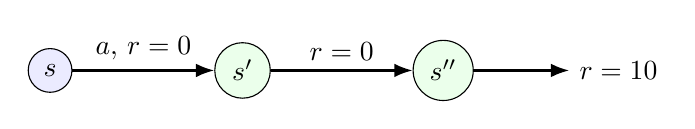
\begin{tikzpicture}[node distance=1.8cm, arrow/.style={-Latex, thick}]
\node[draw, circle, fill=blue!8] (s0) {$s$};
\node[draw, circle, fill=green!8, right=of s0] (s1) {$s'$};
\node[draw, circle, fill=green!8, right=of s1] (s2) {$s''$};
\draw[arrow] (s0) -- node[above] {$a,\, r=0$} (s1);
\draw[arrow] (s1) -- node[above] {$r=0$} (s2);
\draw[arrow] (s2) -- ++(1.6,0) node[right] {$r=10$};
\end{tikzpicture}
\end{center}

\vspace{0.5em}
The action at $s$ matters because it changes the distribution of future rewards.
\end{frame}

\begin{frame}{Exploration Versus Exploitation}
\small
\begin{itemize}
    \item \red{Exploitation}: choose actions that look best under current estimates.
    \item \red{Exploration}: choose actions to improve future estimates.
    \item RL requires both because the data distribution is controlled by the policy.
\end{itemize}

\vspace{0.8em}
\[
\text{Let }a^*(s)\in\argmax_b Q(s,b),\qquad
\epsilon\text{-greedy:}\quad
\pi(a\mid s)=
\begin{cases}
1-\epsilon+\epsilon/|\Aspace(s)|, & a=a^*(s),\\
\epsilon/|\Aspace(s)|, & \text{otherwise.}
\end{cases}
\]

\vspace{0.4em}
This simple rule is often enough to expose the exploration issue clearly.
\end{frame}

\begin{frame}{Prediction and Control}
\small
\begin{columns}[T,onlytextwidth]
\begin{column}{0.48\textwidth}
\textbf{Prediction}
\begin{itemize}
    \item Policy $\pi$ is fixed.
    \item Learn $v_\pi$ or $q_\pi$.
    \item Question: how good is this behavior?
\end{itemize}
\end{column}
\begin{column}{0.48\textwidth}
\textbf{Control}
\begin{itemize}
    \item Policy changes during learning.
    \item Learn values and improve policy.
    \item Question: how should the agent behave?
\end{itemize}
\end{column}
\end{columns}

\vspace{1em}
\begin{block}{Main algorithmic pattern}
Most tabular control algorithms repeatedly alternate between value estimation and policy improvement.
\end{block}
\end{frame}

\begin{frame}{Model-Based and Model-Free}
\small
\begin{tabular}{>{\raggedright\arraybackslash}p{0.24\textwidth}
                >{\raggedright\arraybackslash}p{0.32\textwidth}
                >{\raggedright\arraybackslash}p{0.32\textwidth}}
\toprule
Approach & What is learned or known & How actions improve \\
\midrule
Model-based & Estimate or use $p(s',r\mid s,a)$ & Plan by simulating backups \\
Model-free & Estimate $v_\pi$ or $q_\pi$ directly & Improve policy from value estimates \\
Policy search & Parameterize $\pi_\theta$ directly & Optimize expected return \\
\bottomrule
\end{tabular}

\vspace{1em}
Sutton--Barto Chapters 6 and 7 focus on model-free value learning in the tabular setting.
\end{frame}

\begin{frame}{Tic-Tac-Toe as the First Value-Learning Picture}
\small
\begin{itemize}
    \item Keep a table with one number for each board position.
    \item Interpret the number as the current estimate of eventual win probability.
    \item Pick moves that lead to high-value positions, with occasional exploration.
    \item After the game, adjust earlier values toward later values and outcomes.
\end{itemize}

\vspace{0.7em}
\[
V(S_t) \leftarrow V(S_t)+\alpha\bigl[V(S_{t+1})-V(S_t)\bigr]
\]

\vspace{0.4em}
This is the seed of the backup idea: later estimates teach earlier estimates.
\end{frame}

\section{Finite Markov Decision Processes}

\begin{frame}{Finite MDP}
\small
A finite Markov decision process is specified by
\[
(\Sspace,\Aspace,p,\gamma),
\qquad
p(s',r\mid s,a)=\PP(S_{t+1}=s',R_{t+1}=r\mid S_t=s,A_t=a).
\]

\begin{itemize}
    \item $\Sspace$: finite state set.
    \item $\Aspace(s)$: finite action set available in state $s$.
    \item $p$: one-step transition and reward law.
    \item $\gamma\in[0,1]$: discount factor.
\end{itemize}

\vspace{0.5em}
Once $p$ is known and the state is Markov, all future prediction can be built from one-step dynamics.
\end{frame}

\begin{frame}{The Markov Property}
\small
\[
\PP(S_{t+1}=s',R_{t+1}=r \mid S_0,A_0,R_1,\ldots,S_t,A_t)
=p(s',r\mid S_t,A_t).
\]

\vspace{0.7em}
\begin{itemize}
    \item The current state contains all history that is useful for predicting the next step.
    \item Markov does not mean the state contains every physical fact.
    \item It means no forgotten history would improve the conditional distribution relevant to the task.
\end{itemize}

\vspace{0.7em}
\begin{block}{Practical reading}
In real systems, the state representation is often only approximately Markov; the theory tells us what information the representation should try to preserve.
\end{block}
\end{frame}

\begin{frame}{Dynamics Decompositions}
\small
From the joint one-step law,
\[
p(s',r\mid s,a),
\]
we often use derived quantities:
\[
p(s'\mid s,a)=\sum_{r\in\Rspace}p(s',r\mid s,a),
\]
\[
r(s,a)=\EE[R_{t+1}\mid S_t=s,A_t=a]
      =\sum_{s',r} r\,p(s',r\mid s,a),
\]
\[
r(s,a,s')=\EE[R_{t+1}\mid S_t=s,A_t=a,S_{t+1}=s'].
\]

The joint form is the cleanest because reward and next state can be statistically coupled.
\end{frame}

\begin{frame}{Policies}
\small
A policy defines behavior:
\[
\pi(a\mid s)=\PP(A_t=a\mid S_t=s).
\]

\begin{itemize}
    \item Deterministic policy: $\pi(s)\in\Aspace(s)$.
    \item Stochastic policy: distribution over actions.
    \item Stationary policy: same mapping at every time step.
\end{itemize}

\vspace{0.8em}
Given an MDP and a policy $\pi$, the interaction becomes a Markov reward process. Prediction is then well-defined.
\end{frame}

\begin{frame}{Return: The Quantity We Optimize}
\small
The return from time $t$ is the discounted sum of future rewards:
\[
G_t = R_{t+1}+\gamma R_{t+2}+\gamma^2 R_{t+3}+\cdots
    = \sum_{k=0}^{\infty}\gamma^k R_{t+k+1}.
\]

\begin{itemize}
    \item Episodic tasks can terminate; terminal states produce no further reward.
    \item Continuing tasks often require $\gamma<1$ to make the infinite sum finite.
    \item $\gamma=0$ is myopic; $\gamma\rightarrow 1$ is farsighted.
\end{itemize}
\end{frame}

\begin{frame}{Episodic and Continuing Tasks}
\small
\begin{columns}[T,onlytextwidth]
\begin{column}{0.48\textwidth}
\textbf{Episodic}
\begin{itemize}
    \item Interaction breaks into episodes.
    \item Examples: games, trips through a maze.
    \item Return can be finite even with $\gamma=1$.
\end{itemize}
\[
G_t=\sum_{k=0}^{T-t-1}\gamma^k R_{t+k+1}.
\]
\end{column}
\begin{column}{0.48\textwidth}
\textbf{Continuing}
\begin{itemize}
    \item No natural terminal time.
    \item Examples: process control, long-lived robot.
    \item Discounting is the standard finite-return device.
\end{itemize}
\[
G_t=\sum_{k=0}^{\infty}\gamma^k R_{t+k+1}.
\]
\end{column}
\end{columns}
\end{frame}

\begin{frame}{Reward Design: The Objective Boundary}
\small
\begin{itemize}
    \item The reward signal defines the task, not the algorithm.
    \item It should represent what we want the agent to achieve, not how we want it to achieve it.
    \item Bad reward design creates policies that optimize the signal while missing the intent.
\end{itemize}

\vspace{0.8em}
\begin{block}{Useful rule}
Reward is the external objective. Value is the agent's learned prediction of that objective under a policy.
\end{block}
\end{frame}

\begin{frame}{State-Value Function}
\small
For a policy $\pi$, the value of state $s$ is
\[
v_\pi(s)
=\EE_\pi[G_t\mid S_t=s].
\]

\begin{itemize}
    \item It answers: if we start here and follow $\pi$, how much return should we expect?
    \item It is a prediction problem once $\pi$ is fixed.
    \item It is the central object behind policy evaluation.
\end{itemize}
\end{frame}

\begin{frame}{Action-Value Function}
\small
For a policy $\pi$, the value of taking action $a$ in state $s$ is
\[
q_\pi(s,a)
=\EE_\pi[G_t\mid S_t=s,A_t=a].
\]

\begin{itemize}
    \item It answers: what if we force the first action to be $a$, then follow $\pi$?
    \item It is more directly useful for control when the model is unknown.
    \item A greedy policy can be read directly from $q$:
    \[
    \pi_{\text{greedy}}(s)\in\argmax_a q(s,a).
    \]
\end{itemize}
\end{frame}

\begin{frame}{Bellman Expectation Equation for $v_\pi$}
\small
Split return into one reward plus discounted future return:
\[
G_t=R_{t+1}+\gamma G_{t+1}.
\]

Therefore
\[
v_\pi(s)=
\sum_{a}\pi(a\mid s)\sum_{s',r}p(s',r\mid s,a)
\bigl[r+\gamma v_\pi(s')\bigr].
\]

\vspace{0.6em}
\begin{block}{Interpretation}
Value is self-consistent: it equals expected immediate reward plus discounted value of the next state.
\end{block}
\end{frame}

\begin{frame}{Bellman Expectation Equation for $q_\pi$}
\small
\[
q_\pi(s,a)=
\sum_{s',r}p(s',r\mid s,a)
\left[
r+\gamma\sum_{a'}\pi(a'\mid s')q_\pi(s',a')
\right].
\]

\vspace{0.8em}
\begin{itemize}
    \item The first action is fixed to $a$.
    \item At the next state, actions follow $\pi$.
    \item This equation underlies Sarsa.
\end{itemize}
\end{frame}

\begin{frame}{Optimal Value Functions}
\small
\[
v_*(s)=\max_\pi v_\pi(s),
\qquad
q_*(s,a)=\max_\pi q_\pi(s,a).
\]

\vspace{0.6em}
\begin{itemize}
    \item $v_*$ tells us the best achievable return from a state.
    \item $q_*$ tells us the best achievable return after a specified first action.
    \item Any policy greedy with respect to $q_*$ is optimal:
    \[
    \pi_*(s)\in\argmax_a q_*(s,a).
    \]
\end{itemize}
\end{frame}

\begin{frame}{Bellman Optimality Equations}
\small
\[
v_*(s)=
\max_a \sum_{s',r}p(s',r\mid s,a)
\bigl[r+\gamma v_*(s')\bigr],
\]
\[
q_*(s,a)=
\sum_{s',r}p(s',r\mid s,a)
\bigl[r+\gamma\max_{a'}q_*(s',a')\bigr].
\]

\vspace{0.6em}
\begin{block}{Control as fixed-point search}
Finding an optimal policy can be reduced to finding the fixed point of an optimal Bellman backup.
\end{block}
\end{frame}

\begin{frame}{Bellman Equation as a Fixed-Point Problem}
\small
\textbf{For a fixed policy} $\pi$, the Bellman expectation equation is a linear system:
\[
\mathbf{v}_\pi=\mathbf{r}_\pi+\gamma P_\pi \mathbf{v}_\pi,
\qquad
(I-\gamma P_\pi)\mathbf{v}_\pi=\mathbf{r}_\pi.
\]
\[
\mathbf{v}_\pi=(I-\gamma P_\pi)^{-1}\mathbf{r}_\pi
\quad \text{if the inverse is feasible to compute.}
\]

\vspace{0.6em}
\textbf{For control}, the optimal Bellman equation is nonlinear:
\[
v_* = T_* v_*,
\qquad
(T_*V)(s)=\max_a\sum_{s',r}p(s',r\mid s,a)\bigl[r+\gamma V(s')\bigr].
\]

\vspace{0.4em}
Policy iteration and value iteration are practical ways to solve these Bellman fixed-point equations.
\end{frame}

\begin{frame}{Backup Diagrams Without the Diagrams}
\small
Almost every tabular RL algorithm can be understood by three choices:

\begin{enumerate}
    \item \red{What target?} full return, one-step bootstrapped target, or multi-step mixture.
    \item \red{What expectation?} exact expectation over $p$, sample transition, or sampled episode.
    \item \red{What policy?} evaluate current policy, behave with another policy, or improve greedily.
\end{enumerate}

\vspace{0.8em}
\[
\text{old estimate} \leftarrow
\text{old estimate}+\alpha(\text{target}-\text{old estimate}).
\]
\end{frame}

\section{The Algorithmic Bridge: Evaluation and Improvement}

\begin{frame}{Policy Evaluation}
\small
Given policy $\pi$, estimate $v_\pi$.

\vspace{0.5em}
\textbf{Dynamic programming update when $p$ is known:}
\[
V_{k+1}(s)=
\sum_a \pi(a\mid s)\sum_{s',r}p(s',r\mid s,a)
\bigl[r+\gamma V_k(s')\bigr].
\]

\vspace{0.7em}
This is a full-width Bellman expectation backup: average over all actions, next states, and rewards.
\end{frame}

\begin{frame}{Policy Improvement}
\small
Given $v_\pi$, choose actions greedily with respect to one-step lookahead:
\[
\pi'(s)\in\argmax_a
\sum_{s',r}p(s',r\mid s,a)\bigl[r+\gamma v_\pi(s')\bigr].
\]

\vspace{0.7em}
\begin{itemize}
    \item If $\pi'$ is greedy with respect to $v_\pi$, then it is no worse than $\pi$.
    \item Repeating evaluation and improvement leads to policy iteration.
\end{itemize}
\end{frame}

\begin{frame}{Generalized Policy Iteration}
\centering
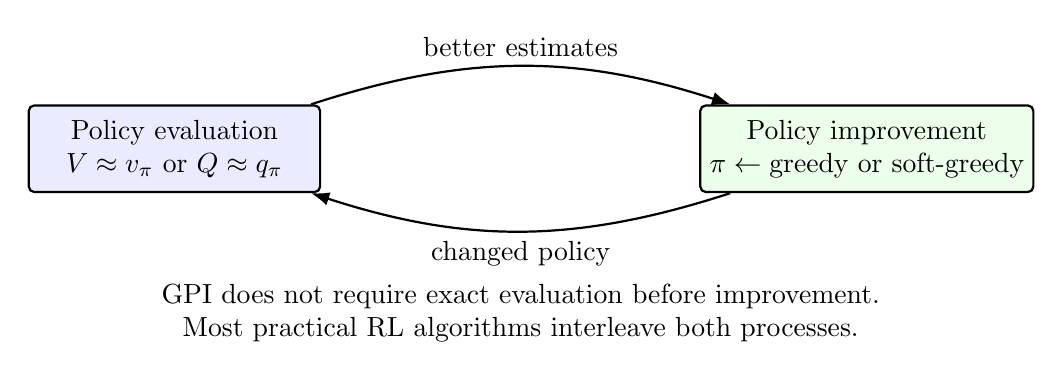
\begin{tikzpicture}[
    box/.style={draw, rounded corners=2pt, minimum width=3.7cm, minimum height=1.1cm, align=center, thick},
    arrow/.style={-Latex, thick}
]
\node[box, fill=blue!8] (eval) {Policy evaluation\\$V\approx v_\pi$ or $Q\approx q_\pi$};
\node[box, fill=green!8, right=4.8cm of eval] (imp) {Policy improvement\\$\pi \leftarrow \text{greedy or soft-greedy}$};
\draw[arrow, bend left=18] (eval) to node[above] {better estimates} (imp);
\draw[arrow, bend left=18] (imp) to node[below] {changed policy} (eval);
\node[below=1.6cm of $(eval)!0.5!(imp)$, align=center] {
GPI does not require exact evaluation before improvement.\\
Most practical RL algorithms interleave both processes.
};
\end{tikzpicture}
\end{frame}

\begin{frame}{How Evaluation and Improvement Alternate}
\small
\begin{columns}[T,onlytextwidth]
\begin{column}{0.48\textwidth}
\textbf{Exact policy iteration}
\begin{enumerate}
    \item Fix $\pi_k$.
    \item Evaluate until $V\approx v_{\pi_k}$ is accurate.
    \item Improve once:
    \[
    \pi_{k+1}(s)\in\argmax_a q_{\pi_k}(s,a).
    \]
\end{enumerate}
\end{column}
\begin{column}{0.48\textwidth}
\textbf{Generalized policy iteration}
\begin{enumerate}
    \item Do a few value updates.
    \item Improve the policy a little.
    \item Repeat without waiting for full convergence.
\end{enumerate}
\end{column}
\end{columns}

\vspace{0.8em}
\begin{block}{Main point}
Policy evaluation asks ``how good is the current policy?'' Policy improvement asks ``how should the policy change given these values?''
\end{block}
\end{frame}

\begin{frame}{Solving Bellman Equations: Policy and Value Iteration}
\small
\begin{columns}[T,onlytextwidth]
\begin{column}{0.48\textwidth}
\textbf{Policy iteration solves}
\[
v_{\pi_k}=T_{\pi_k}v_{\pi_k}
\]
\begin{enumerate}
    \item Evaluate $v_{\pi_k}$.
    \item Improve $\pi_k$ greedily.
    \item Stop when policy is stable.
\end{enumerate}
\end{column}
\begin{column}{0.48\textwidth}
\textbf{Value iteration solves}
\[
v_*=T_*v_*
\]
\[
V_{k+1}(s)=\max_a\sum_{s',r}p(s',r\mid s,a)
\bigl[r+\gamma V_k(s')\bigr].
\]
Evaluation and improvement are merged into one optimality backup.
\end{column}
\end{columns}

\vspace{0.8em}
These methods are exact dynamic programming solvers when $p$ is known.
\end{frame}

\begin{frame}{Monte Carlo Evaluation}
\small
If the model is unknown but complete episodes are available:
\[
V(S_t)\leftarrow V(S_t)+\alpha\bigl[G_t-V(S_t)\bigr].
\]

\begin{itemize}
    \item No bootstrapping: the target is an observed return.
    \item No model: uses sampled experience.
    \item Naturally episodic: must wait until enough future reward is observed.
\end{itemize}

\vspace{0.6em}
Monte Carlo is simple, unbiased for the value under the sampled policy, and can have high variance.
\end{frame}

\begin{frame}{DP, MC, and TD: The Three Backup Styles}
\small
\setlength{\tabcolsep}{4pt}
\begin{tabular}{>{\raggedright\arraybackslash}p{0.17\textwidth}
                >{\raggedright\arraybackslash}p{0.26\textwidth}
                >{\raggedright\arraybackslash}p{0.21\textwidth}
                >{\raggedright\arraybackslash}p{0.20\textwidth}}
\toprule
Method & Target & Model needed? & Wait for episode end? \\
\midrule
Dynamic programming & Expected Bellman target & Yes & No \\
Monte Carlo & Sampled full return $G_t$ & No & Usually yes \\
Temporal difference & Sampled bootstrapped target & No & No \\
\bottomrule
\end{tabular}

\vspace{1em}
\[
\text{TD target}=R_{t+1}+\gamma V(S_{t+1}).
\]
\end{frame}

\begin{frame}{Sampling and Bootstrapping}
\small
\begin{columns}[T,onlytextwidth]
\begin{column}{0.48\textwidth}
\textbf{Sampling}
\begin{itemize}
    \item Use experienced transitions.
    \item Avoid summing over all next states.
    \item Introduces sampling noise.
\end{itemize}
\end{column}
\begin{column}{0.48\textwidth}
\textbf{Bootstrapping}
\begin{itemize}
    \item Use current value estimate in the target.
    \item Learn before final outcome is known.
    \item Introduces bias from current estimates.
\end{itemize}
\end{column}
\end{columns}

\vspace{1em}
TD learning is the central combination: \red{sampled transitions plus bootstrapped targets}.
\end{frame}

\section{Temporal-Difference Learning}

\begin{frame}{TD Prediction}
\small
TD(0) updates after each transition:
\[
V(S_t)\leftarrow V(S_t)+\alpha\delta_t,
\]
where
\[
\delta_t=R_{t+1}+\gamma V(S_{t+1})-V(S_t).
\]

\vspace{0.7em}
\begin{itemize}
    \item $\delta_t$ is the temporal-difference error.
    \item It measures surprise relative to the current one-step prediction.
    \item It is also the learning signal used in many actor--critic algorithms.
\end{itemize}
\end{frame}

\begin{frame}{TD(0) Algorithm}
\small
\textbf{Input:} policy $\pi$, step size $\alpha$, initial $V$.

\vspace{0.5em}
\begin{enumerate}
    \item Initialize $S$ at the start of an episode.
    \item Choose $A\sim\pi(\cdot\mid S)$.
    \item Take action $A$, observe $R$ and $S'$.
    \item Update
    \[
    V(S)\leftarrow V(S)+\alpha\bigl[R+\gamma V(S')-V(S)\bigr].
    \]
    \item Set $S\leftarrow S'$ and continue until termination.
\end{enumerate}

\vspace{0.4em}
For terminal $S'$, use $V(S')=0$.
\end{frame}

\begin{frame}{Why TD Is Between MC and DP}
\small
\begin{tabular}{>{\raggedright\arraybackslash}p{0.24\textwidth}
                >{\raggedright\arraybackslash}p{0.30\textwidth}
                >{\raggedright\arraybackslash}p{0.30\textwidth}}
\toprule
Property & Monte Carlo & TD(0) \\
\midrule
Target & $G_t$ & $R_{t+1}+\gamma V(S_{t+1})$ \\
Uses samples? & Yes & Yes \\
Bootstraps? & No & Yes \\
Online update? & Only after return known & Immediately \\
Variance & Higher & Lower \\
Bias from estimate & Lower & Higher \\
\bottomrule
\end{tabular}
\end{frame}

\begin{frame}{Random Walk Example}
\small
\begin{center}
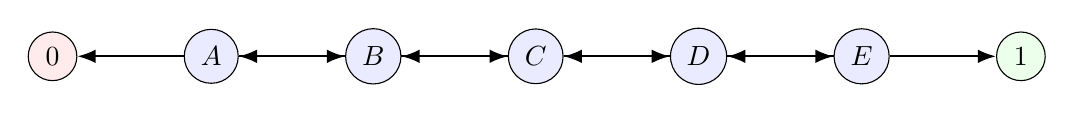
\begin{tikzpicture}[node distance=1.35cm, arrow/.style={-Latex, thick}]
\node[draw, circle, fill=red!8] (L) {$0$};
\node[draw, circle, fill=blue!8, right=of L] (A) {$A$};
\node[draw, circle, fill=blue!8, right=of A] (B) {$B$};
\node[draw, circle, fill=blue!8, right=of B] (C) {$C$};
\node[draw, circle, fill=blue!8, right=of C] (D) {$D$};
\node[draw, circle, fill=blue!8, right=of D] (E) {$E$};
\node[draw, circle, fill=green!8, right=of E] (R) {$1$};
\draw[arrow] (A) -- (L);
\draw[arrow] (A) -- (B);
\draw[arrow] (B) -- (A);
\draw[arrow] (B) -- (C);
\draw[arrow] (C) -- (B);
\draw[arrow] (C) -- (D);
\draw[arrow] (D) -- (C);
\draw[arrow] (D) -- (E);
\draw[arrow] (E) -- (D);
\draw[arrow] (E) -- (R);
\end{tikzpicture}
\end{center}

\vspace{0.6em}
\begin{itemize}
    \item Start in $C$; move left or right with equal probability.
    \item Reward is $1$ only when terminating on the right.
    \item True values are probabilities of eventual right termination.
\end{itemize}

\vspace{0.4em}
TD updates intermediate states before the final terminal reward has been fully propagated by Monte Carlo averaging.
\end{frame}

\begin{frame}{Batch TD Intuition}
\small
With a fixed batch of experience:

\begin{itemize}
    \item Monte Carlo estimates values that fit the observed returns in the batch.
    \item TD(0) estimates values that are consistent with the maximum-likelihood Markov model induced by the batch.
\end{itemize}

\vspace{0.9em}
\begin{block}{Why this matters}
If the Markov assumption is right, TD can generalize across repeated transitions: a transition from $A$ to $B$ teaches $A$ through the current estimate of $B$.
\end{block}
\end{frame}

\begin{frame}{From State Values to Action Values}
\small
For control without a model, it is convenient to learn $Q(s,a)$.

\vspace{0.5em}
\[
Q(S_t,A_t)\leftarrow Q(S_t,A_t)+\alpha(\text{target}-Q(S_t,A_t)).
\]

\vspace{0.5em}
\begin{itemize}
    \item If the target follows the actually selected next action, we get \red{Sarsa}.
    \item If the target uses the greedy next action, we get \red{Q-learning}.
    \item The difference is the difference between on-policy and off-policy control.
\end{itemize}
\end{frame}

\begin{frame}{Sarsa: On-Policy TD Control}
\small
The update uses the quintuple $(S_t,A_t,R_{t+1},S_{t+1},A_{t+1})$:
\[
Q(S_t,A_t)\leftarrow Q(S_t,A_t)+\alpha
\left[
R_{t+1}+\gamma Q(S_{t+1},A_{t+1})-Q(S_t,A_t)
\right].
\]

\vspace{0.7em}
\begin{itemize}
    \item Behavior policy and target policy are the same.
    \item Usually use $\epsilon$-greedy policy derived from $Q$.
    \item Learns the value of the exploratory policy it actually follows.
\end{itemize}
\end{frame}

\begin{frame}{Sarsa Algorithm}
\small
\begin{enumerate}
    \item Initialize $Q(s,a)$.
    \item For each episode, initialize $S$ and choose $A$ from the current policy.
    \item Take $A$, observe $R,S'$.
    \item Choose $A'$ from the current policy at $S'$.
    \item Update
    \[
    Q(S,A)\leftarrow Q(S,A)+\alpha[R+\gamma Q(S',A')-Q(S,A)].
    \]
    \item Set $S\leftarrow S'$, $A\leftarrow A'$ and repeat.
\end{enumerate}
\end{frame}

\begin{frame}{Q-Learning: Off-Policy TD Control}
\small
The update uses the greedy value of the next state:
\[
Q(S_t,A_t)\leftarrow Q(S_t,A_t)+\alpha
\left[
R_{t+1}+\gamma\max_{a}Q(S_{t+1},a)-Q(S_t,A_t)
\right].
\]

\vspace{0.7em}
\begin{itemize}
    \item Behavior policy may be exploratory.
    \item Target policy is greedy with respect to $Q$.
    \item Learns an approximation to $q_*$ while behaving non-greedily.
\end{itemize}
\end{frame}

\begin{frame}{Q-Learning Algorithm}
\small
\begin{enumerate}
    \item Initialize $Q(s,a)$.
    \item For each episode, initialize $S$.
    \item Choose $A$ from a behavior policy, e.g. $\epsilon$-greedy from $Q$.
    \item Take $A$, observe $R,S'$.
    \item Update
    \[
    Q(S,A)\leftarrow Q(S,A)+\alpha[R+\gamma\max_a Q(S',a)-Q(S,A)].
    \]
    \item Set $S\leftarrow S'$ and repeat.
\end{enumerate}
\end{frame}

\begin{frame}{Sarsa Versus Q-Learning}
\small
\begin{tabular}{>{\raggedright\arraybackslash}p{0.23\textwidth}
                >{\raggedright\arraybackslash}p{0.32\textwidth}
                >{\raggedright\arraybackslash}p{0.32\textwidth}}
\toprule
Question & Sarsa & Q-learning \\
\midrule
Policy type & On-policy & Off-policy \\
Target & $R+\gamma Q(S',A')$ & $R+\gamma\max_a Q(S',a)$ \\
Learns value of & Exploratory behavior policy & Greedy target policy \\
Risk-sensitive effect & Accounts for exploratory actions & Ignores future exploration in target \\
\bottomrule
\end{tabular}
\end{frame}

\begin{frame}{Cliff-Walking Intuition}
\small
\begin{itemize}
    \item The shortest path near a cliff is optimal for a perfectly greedy policy.
    \item With $\epsilon$-greedy exploration, the agent sometimes slips into bad actions.
    \item Sarsa evaluates the policy including these exploratory slips.
    \item Q-learning evaluates the greedy policy while still using exploratory behavior.
\end{itemize}

\vspace{0.9em}
\begin{block}{Takeaway}
On-policy methods optimize what the agent actually does; off-policy methods can learn about a different target policy from exploratory data.
\end{block}
\end{frame}

\begin{frame}{Expected Sarsa as a Useful Middle Point}
\small
Expected Sarsa replaces the sampled next action by its expectation:
\[
Q(S_t,A_t)\leftarrow Q(S_t,A_t)+\alpha
\left[
R_{t+1}+\gamma\sum_a\pi(a\mid S_{t+1})Q(S_{t+1},a)-Q(S_t,A_t)
\right].
\]

\vspace{0.7em}
\begin{itemize}
    \item Same target policy idea as Sarsa.
    \item Lower variance than sampling $A_{t+1}$.
    \item Becomes Q-learning when $\pi$ is greedy in the target.
\end{itemize}
\end{frame}

\begin{frame}{Convergence Conditions in the Tabular Case}
\small
For one-step tabular control, convergence statements usually require:

\begin{itemize}
    \item finite state and action spaces;
    \item sufficient exploration: all relevant state--action pairs visited infinitely often;
    \item decreasing step sizes such as
    \[
    \sum_t \alpha_t(s,a)=\infty,\qquad
    \sum_t \alpha_t(s,a)^2<\infty;
    \]
    \item for on-policy control, policies become greedy in the limit while still exploring enough.
\end{itemize}

\vspace{0.5em}
Constant step sizes are common in nonstationary or approximate settings, but exact convergence guarantees change.
\end{frame}

\section{Multi-Step Returns and Eligibility Traces}

\begin{frame}{Why One-Step TD Is Not Enough}
\small
One-step TD assigns each reward through one transition at a time:
\[
R_{t+1}+\gamma V(S_{t+1}).
\]

\vspace{0.7em}
\begin{itemize}
    \item It is online and low variance.
    \item But reward information may propagate slowly over long horizons.
    \item Monte Carlo uses the full outcome but waits and has higher variance.
\end{itemize}

\vspace{0.7em}
Chapter 7 introduces a spectrum between these extremes.
\end{frame}

\begin{frame}{$n$-Step Return}
\small
The $n$-step return bootstraps after $n$ rewards:
\[
G_{t:t+n}=
R_{t+1}+\gamma R_{t+2}+\cdots+\gamma^{n-1}R_{t+n}
\,+\,\gamma^n V(S_{t+n}).
\]

\vspace{0.7em}
\[
V(S_t)\leftarrow V(S_t)+\alpha\bigl[G_{t:t+n}-V(S_t)\bigr].
\]

\vspace{0.6em}
\begin{itemize}
    \item $n=1$: TD(0).
    \item $n$ reaches terminal time: Monte Carlo target.
\end{itemize}
\end{frame}

\begin{frame}{Choosing $n$}
\small
\begin{columns}[T,onlytextwidth]
\begin{column}{0.48\textwidth}
\textbf{Small $n$}
\begin{itemize}
    \item More bootstrapping.
    \item Lower variance.
    \item Faster online updates.
    \item More bias from current estimates.
\end{itemize}
\end{column}
\begin{column}{0.48\textwidth}
\textbf{Large $n$}
\begin{itemize}
    \item Less bootstrapping.
    \item More real reward information.
    \item Higher variance.
    \item Slower credit assignment online.
\end{itemize}
\end{column}
\end{columns}

\vspace{0.8em}
TD($\lambda$) avoids choosing just one $n$ by averaging many $n$-step returns.
\end{frame}

\begin{frame}{Forward View of TD($\lambda$)}
\small
The $\lambda$-return is an exponentially weighted average of $n$-step returns:
\[
G_t^\lambda=(1-\lambda)\sum_{n=1}^{\infty}\lambda^{n-1}G_{t:t+n}.
\]

\vspace{0.7em}
For episodic tasks with terminal time $T$:
\[
G_t^\lambda=(1-\lambda)\sum_{n=1}^{T-t-1}\lambda^{n-1}G_{t:t+n}
\,+\,\lambda^{T-t-1}G_t.
\]

\vspace{0.4em}
Then update toward $G_t^\lambda$:
\[
V(S_t)\leftarrow V(S_t)+\alpha\bigl[G_t^\lambda-V(S_t)\bigr].
\]
\end{frame}

\begin{frame}{Endpoints of $\lambda$}
\small
\begin{itemize}
    \item If $\lambda=0$:
    \[
    G_t^\lambda=G_{t:t+1}=R_{t+1}+\gamma V(S_{t+1}),
    \]
    so TD($\lambda$) becomes TD(0).
    \item If $\lambda=1$ in an episodic task:
    \[
    G_t^\lambda=G_t,
    \]
    so the target becomes the Monte Carlo return.
\end{itemize}

\vspace{0.7em}
$\lambda$ controls the degree of bootstrapping.
\end{frame}

\begin{frame}{Forward View Is Conceptual, Not Causal}
\small
The forward view asks:

\vspace{0.3em}
\begin{center}
\emph{For the state visited at time $t$, what sequence of future rewards and future estimates should determine its update?}
\end{center}

\vspace{0.8em}
\begin{itemize}
    \item It explains the target.
    \item But it needs future rewards before updating $S_t$.
    \item The backward view gives a causal implementation using eligibility traces.
\end{itemize}
\end{frame}

\begin{frame}{Eligibility Trace}
\small
For each state $s$, maintain a trace $E_t(s)$ measuring recent visitation.

\[
E_t(s)=\gamma\lambda E_{t-1}(s)+\one\{S_t=s\}.
\]

\vspace{0.8em}
\begin{itemize}
    \item Recently visited states have large traces.
    \item Traces decay by $\gamma\lambda$.
    \item The current TD error updates all states in proportion to their traces.
\end{itemize}
\end{frame}

\begin{frame}{Backward View of TD($\lambda$)}
\small
Compute the one-step TD error:
\[
\delta_t=R_{t+1}+\gamma V(S_{t+1})-V(S_t).
\]

Update every state:
\[
V(s)\leftarrow V(s)+\alpha\delta_t E_t(s),
\qquad \forall s\in\Sspace.
\]

\vspace{0.8em}
\begin{block}{Mechanism}
When a surprising reward or transition occurs now, the trace sends credit backward to states visited recently.
\end{block}
\end{frame}

\begin{frame}{TD($\lambda$) Algorithm}
\small
\begin{enumerate}
    \item Initialize $V(s)$.
    \item At the start of each episode, set $E(s)=0$ for all $s$.
    \item At each step, observe $S,A,R,S'$ under policy $\pi$.
    \item Compute $\delta=R+\gamma V(S')-V(S)$.
    \item Increase the trace of the visited state: $E(S)\leftarrow E(S)+1$.
    \item For all $s$:
    \[
    V(s)\leftarrow V(s)+\alpha\delta E(s),
    \qquad
    E(s)\leftarrow\gamma\lambda E(s).
    \]
\end{enumerate}
\end{frame}

\begin{frame}{Accumulating and Replacing Traces}
\small
\begin{columns}[T,onlytextwidth]
\begin{column}{0.48\textwidth}
\textbf{Accumulating trace}
\[
E(S_t)\leftarrow E(S_t)+1.
\]
\begin{itemize}
    \item Multiple close visits accumulate.
    \item Natural from the classical derivation.
\end{itemize}
\end{column}
\begin{column}{0.48\textwidth}
\textbf{Replacing trace}
\[
E(S_t)\leftarrow 1.
\]
\begin{itemize}
    \item Caps the active state's trace.
    \item Often useful in tabular tasks with loops.
\end{itemize}
\end{column}
\end{columns}

\vspace{0.7em}
Both express the same idea: eligibility is a fading memory of recent responsibility.
\end{frame}

\begin{frame}{Sarsa($\lambda$)}
\small
Use traces over state--action pairs:
\[
E_t(s,a)=\gamma\lambda E_{t-1}(s,a)+\one\{S_t=s,A_t=a\}.
\]

The TD error is the Sarsa error:
\[
\delta_t=R_{t+1}+\gamma Q(S_{t+1},A_{t+1})-Q(S_t,A_t).
\]

Update all pairs:
\[
Q(s,a)\leftarrow Q(s,a)+\alpha\delta_t E_t(s,a).
\]
\end{frame}

\begin{frame}{Sarsa($\lambda$) Algorithm}
\small
\begin{enumerate}
    \item Initialize $Q(s,a)$.
    \item At episode start, set all $E(s,a)=0$.
    \item Choose $A$ from the current behavior policy.
    \item Take $A$, observe $R,S'$, choose $A'$.
    \item Compute $\delta=R+\gamma Q(S',A')-Q(S,A)$.
    \item Set $E(S,A)\leftarrow E(S,A)+1$.
    \item For all $(s,a)$:
    \[
    Q(s,a)\leftarrow Q(s,a)+\alpha\delta E(s,a),
    \qquad
    E(s,a)\leftarrow\gamma\lambda E(s,a).
    \]
\end{enumerate}
\end{frame}

\begin{frame}{Watkins's Q($\lambda$)}
\small
Q-learning can also be combined with traces:
\[
\delta_t=R_{t+1}+\gamma\max_a Q(S_{t+1},a)-Q(S_t,A_t).
\]

\vspace{0.6em}
\begin{itemize}
    \item If the next action is greedy, traces continue.
    \item If the next action is exploratory, traces are cut off.
    \item Reason: off-policy backups should not credit earlier actions through a later action that deviates from the greedy target policy.
\end{itemize}

\vspace{0.5em}
This is an early example of the extra care needed for off-policy multi-step learning.
\end{frame}

\begin{frame}{How to Read $\lambda$ Practically}
\small
\begin{itemize}
    \item $\lambda=0$: stable, myopic credit assignment, low variance.
    \item Intermediate $\lambda$: often best empirical tradeoff.
    \item $\lambda\approx 1$: long credit assignment, closer to Monte Carlo, higher variance.
\end{itemize}

\vspace{0.8em}
\begin{block}{Mental model}
$\gamma\lambda$ is the decay rate of memory. A past state remains eligible only while its trace has not faded away.
\end{block}
\end{frame}

\begin{frame}{The Full Tabular Main Line}
\small
\begin{center}
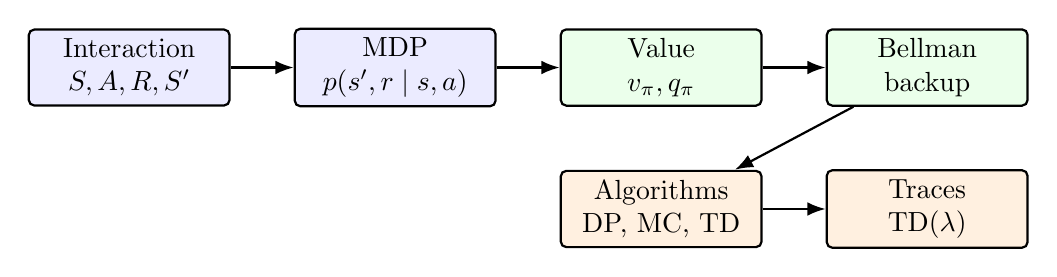
\begin{tikzpicture}[
    box/.style={draw, rounded corners=2pt, minimum width=2.55cm, minimum height=0.9cm, align=center, thick},
    arrow/.style={-Latex, thick}
]
\node[box, fill=blue!8] (rl) {Interaction\\$S,A,R,S'$};
\node[box, fill=blue!8, right=0.8cm of rl] (mdp) {MDP\\$p(s',r\mid s,a)$};
\node[box, fill=green!8, right=0.8cm of mdp] (value) {Value\\$v_\pi,q_\pi$};
\node[box, fill=green!8, right=0.8cm of value] (bellman) {Bellman\\backup};
\node[box, fill=orange!12, below=0.8cm of value] (alg) {Algorithms\\DP, MC, TD};
\node[box, fill=orange!12, right=0.8cm of alg] (traces) {Traces\\TD($\lambda$)};
\draw[arrow] (rl) -- (mdp);
\draw[arrow] (mdp) -- (value);
\draw[arrow] (value) -- (bellman);
\draw[arrow] (bellman) -- (alg);
\draw[arrow] (alg) -- (traces);
\end{tikzpicture}
\end{center}

\vspace{0.7em}
Everything is organized around one idea: estimate long-term value from experience, then use value to improve behavior.
\end{frame}

\section{From Tabular RL to Modern Practice}

\begin{frame}{What Changes with Function Approximation?}
\small
Tabular methods store one number per state or state--action pair.

\[
V(s)\quad \longrightarrow \quad \hat v(s;w),
\qquad
Q(s,a)\quad \longrightarrow \quad \hat q(s,a;w).
\]

\begin{itemize}
    \item Generalization becomes possible across states.
    \item Stability becomes harder because updates couple many states.
    \item The deadly triad appears: function approximation, bootstrapping, and off-policy learning.
\end{itemize}
\end{frame}

\begin{frame}{What Survives in Deep RL?}
\small
\begin{itemize}
    \item The experience tuple $(S_t,A_t,R_{t+1},S_{t+1})$.
    \item The return objective.
    \item Bellman targets and TD errors.
    \item On-policy versus off-policy distinctions.
    \item Multi-step returns and trace-like credit assignment.
    \item Generalized policy iteration: evaluate, improve, repeat.
\end{itemize}

\vspace{0.7em}
DQN, actor--critic, PPO, and many RLHF variants still inherit this conceptual skeleton.
\end{frame}

\begin{frame}{A Minimal Bridge to Policy Gradient}
\small
Value methods improve a policy through value estimates. Policy-gradient methods directly optimize policy parameters:
\[
J(\theta)=\EE_{\tau\sim\pi_\theta}[G_0],
\]
\[
\nabla_\theta J(\theta)
\approx
\EE\left[
\sum_t \nabla_\theta\log\pi_\theta(A_t\mid S_t)\,\widehat{A}_t
\right].
\]

\vspace{0.6em}
\begin{itemize}
    \item $\widehat{A}_t$ is often built from TD errors or multi-step returns.
    \item The value function returns as a critic or baseline.
\end{itemize}
\end{frame}

\begin{frame}{LLM Post-Training Through the RL Lens}
\small
\begin{tabular}{>{\raggedright\arraybackslash}p{0.27\textwidth}
                >{\raggedright\arraybackslash}p{0.55\textwidth}}
\toprule
RL object & LLM post-training analogy \\
\midrule
State $S_t$ & Prompt plus generated context so far \\
Action $A_t$ & Next token or higher-level response decision \\
Policy $\pi_\theta$ & Language model distribution \\
Reward $R$ & Human preference model, rule-based score, task metric \\
Return $G$ & Overall quality or task success of a response/trajectory \\
Value/critic & Learned prediction of future reward or advantage \\
\bottomrule
\end{tabular}

\vspace{0.8em}
The MDP abstraction is still useful, but state/action spaces are enormous and rewards are often learned proxies.
\end{frame}

\begin{frame}{Common Failure Modes}
\small
\begin{itemize}
    \item \red{Reward misspecification}: optimizing the signal instead of the intended goal.
    \item \red{Poor exploration}: never collecting data for better actions.
    \item \red{High variance}: long-horizon returns make learning noisy.
    \item \red{Instability}: bootstrapping plus approximation can diverge.
    \item \red{Distribution shift}: learned values are used on states unlike the data.
\end{itemize}

\vspace{0.7em}
The tabular theory gives clean definitions; modern systems inherit the same issues at scale.
\end{frame}

\section{Summary}

\begin{frame}{The Main Story in Five Equations}
\small
\[
G_t=\sum_{k=0}^{\infty}\gamma^k R_{t+k+1}
\]
\[
v_\pi(s)=\EE_\pi[G_t\mid S_t=s],
\qquad
q_\pi(s,a)=\EE_\pi[G_t\mid S_t=s,A_t=a]
\]
\[
v_\pi(s)=\sum_a\pi(a\mid s)\sum_{s',r}p(s',r\mid s,a)[r+\gamma v_\pi(s')]
\]
\[
\delta_t=R_{t+1}+\gamma V(S_{t+1})-V(S_t)
\]
\[
E_t(s)=\gamma\lambda E_{t-1}(s)+\one\{S_t=s\}.
\]
\end{frame}

\begin{frame}{Algorithm Map}
\small
\begin{tabular}{>{\raggedright\arraybackslash}p{0.22\textwidth}
                >{\raggedright\arraybackslash}p{0.30\textwidth}
                >{\raggedright\arraybackslash}p{0.30\textwidth}}
\toprule
Algorithm family & Target & Main use \\
\midrule
DP evaluation & Expected Bellman target & Known model prediction \\
Value iteration & Bellman optimality target & Known model control \\
Monte Carlo & Full sampled return & Episodic model-free prediction/control \\
TD(0) & One-step sampled Bellman target & Online model-free prediction \\
Sarsa & On-policy action-value TD target & Online exploratory control \\
Q-learning & Greedy off-policy TD target & Learning greedy target policy \\
TD($\lambda$) & Mixture of $n$-step targets & Faster temporal credit assignment \\
\bottomrule
\end{tabular}
\end{frame}

\begin{frame}{Key Takeaways}
\small
\begin{itemize}
    \item RL is about learning behavior from interaction, not just fitting labels.
    \item MDPs make the problem mathematically precise through state, action, transition, reward, and discount.
    \item Value functions transform delayed reward into a local decision score.
    \item Bellman equations are the fixed-point structure behind prediction and control.
    \item TD learning combines sampling and bootstrapping.
    \item Eligibility traces turn one-step TD into multi-step credit assignment.
\end{itemize}
\end{frame}

\begin{frame}{Open Questions}
\small
If you are interested in these questions, please feel free to write an email to me {\color{red}(\href{mailto:hpp@bimsa.cn}{hpp@bimsa.cn})} with your comments.

\begin{enumerate}
    \item How should reward be specified when the true objective is hard to measure?
    \item How can agents explore efficiently in enormous state and action spaces?
    \item Which parts of tabular convergence intuition survive deep function approximation?
    \item How should RL algorithms handle learned, nonstationary reward models?
    \item What is the right abstraction level for RL in language-model agents?
\end{enumerate}
\end{frame}

\begin{frame}{Welcome Inputs}
  \centering
  Any comments?
  \\[2em]
  Welcome your inputs!
\end{frame}

\end{document}
